\documentclass[a4paper,11pt]{report}
% !BIB TS-program = biber
% !BIB program = biber
% Die beiden obigen Zeilen helfen TeXShop auf Mac mit biber
% (Verarbeitung der Bibliographiedatenbank in literatur.bib)



% Diese Datei ist fast vollständig von der Maturaarbeit
%
% Programmierung eines Generators für Trennlinien
% bzw. Schnittkurven von Puzzleteilen
%
% vorgelegt von Luca Bosin im Januar 2019, übernommen.
%
% Ihm sei herzlich gedankt.


% ======== START VON PAKETE LADEN =========
\usepackage[german]{babel}        % Deutschsprachige Beschriftungen
\usepackage[utf8]{inputenc}       % Utf8 Zeichensatz
\usepackage[T1]{fontenc}          % Schriftenkodierung
\usepackage[lighttt]{lmodern}     % Schriftart
\usepackage{amsmath}              % Mathematische Formeln
\usepackage[normalem]{ulem}       % Durchgestrichener Text
\usepackage{xcolor}               % Farbiger Text
\usepackage{verbatim}             % Text ohne Formatierung
\usepackage{listings}             % Code mit Formatierung
\usepackage{csquotes}             % Kontextsensitive Zitatanlage
\usepackage{caption}              % Erweiterte Beschriftungen
\usepackage{subcaption}           % Unterbeschriftungen
\usepackage{geometry}             % Seitenränder
\usepackage{setspace}             % Zeilenabstand
\usepackage{fancyhdr}             % Header und Footer
\usepackage{graphicx}             % Grafiken
\usepackage{wrapfig}
\usepackage{svg}                  % SVG Grafiken
\usepackage{booktabs}             % Tabellen
\usepackage{tabularx}             % Breite von Boxen
\usepackage[style=ieee]{biblatex} % Referenzen
\usepackage{hyperref}             % Hyperlinks im PDF-Dokument
\usepackage{hyperxmp}             % Metadaten im PDF-Dokument
\usepackage{makeidx}              % Optional, für Glossar (Index)
\usepackage[version=4]{mhchem}    % Für chemische Formeln
\usepackage{siunitx}              % Angaben mit Masseinheiten
\makeindex
% ========= ENDE VON PAKETE LADEN =========


% ==== START VON DOKUMENTEIGENSCHAFTEN ==== (Dokument)
\title                   % Titel festlegen
{Vorlage für Maturaarbeiten der KSBG}
\date{34. Oktember 2222 (\today)}   % Datum festlegen 
\author{Ivo Blöchliger, Luca Bosin}  % Autor festlegen
\makeatletter            % Erlaubt das Auslesen der obigen Eigenschaften
\let\papertitle\@title   % Titel in \papertitle speichern
\let\paperdate\@date     % Datum in \paperdate speichern
\let\paperauthor\@author % Autor in \paperauthor speichern
\makeatother
\def\paperinstitution    % Bildungseinrichtung in \paperinstitution speichern
{Kantonsschule am Burggraben St.Gallen}
\def\papertype           % Art dieser Arbeit in \papertype speichern
{Maturaarbeit}
\def\papersupervisor     % Betreuungsperson in \papersupervisor speichern
{Dr. Ivo Blöchliger}
% Achtung: Schlüsselwörter sind weiter unten definiert!
% ==== ENDE VON DOKUMENTEIGENSCHAFTEN =====



% =========================================



% ======= START VON TITEL ANPASSEN ======== (Beschriftungen)
\renewcommand{\lstlistingname}{Quellcode}
\renewcommand{\lstlistlistingname}{Quellcodeverzeichnis}
\DefineBibliographyStrings{german}{bibliography = {Literaturverzeichnis}}
% ======== ENDE VON TITEL ANPASSEN ========



% === START VON SCHRIFTPROBLEME BEHEBEN === (Schriftart)
% Die Schreibmaschinen-Schrift lädt nur den normalen Stil, nicht den fetten oder den kursiven
\ttfamily
\DeclareFontShape{T1}{lmtt}{m}{it}{<->sub*lmtt/m/sl}{}
% === ENDE VON SCHRIFTPROBLEME BEHEBEN ====



% ========= START VON CODEBLÖCKE ========== (Codeblöcke)
\lstset{
  frame=tb,                         % Rahmenlinien (tb = top,bottom)
  language=Java,                    % Programmiersprache (für Syntax-Hervorhebung)
  showstringspaces=false,           % Leerzeichen in Strings ausblenden
  basicstyle=\small\ttfamily,       % Style des Codes
  numbers=left,                     % Position der Zeilennummern
  numberstyle=\tiny\textbf,         % Style der Zeilennummern
  keywordstyle=\textbf,             % Style der Schlüsselwörter
  commentstyle=\color{gray}\textit, % Style der Kommentare
  columns=fullflexible,             % Zeilenumbrüche: Bis an Seitenrand
  breaklines=true,                  % Zeilenumbrüche: Erlauben von Zeilenumbrüchen
  breakatwhitespace=true,           % Zeilenumbrüche: Erlauben von Zeilenumbrüchen bei Leerzeichen
  tabsize=4,                        % Grösse der Tabulatoren (Hard-Tab)
}
% Unterstützung von Sonderzeichen
\lstset{literate=
  {á}{{\'a}}1 {é}{{\'e}}1 {í}{{\'i}}1 {ó}{{\'o}}1 {ú}{{\'u}}1 {Á}{{\'A}}1 {É}{{\'E}}1 
  {Í}{{\'I}}1 {Ó}{{\'O}}1 {Ú}{{\'U}}1 {à}{{\`a}}1 {è}{{\`e}}1 {ì}{{\`i}}1 {ò}{{\`o}}1
  {ù}{{\`u}}1 {À}{{\`A}}1 {È}{{\'E}}1 {Ì}{{\`I}}1 {Ò}{{\`O}}1 {Ù}{{\`U}}1 {ä}{{\"a}}1
  {ë}{{\"e}}1 {ï}{{\"i}}1 {ö}{{\"o}}1 {ü}{{\"u}}1 {Ä}{{\"A}}1 {Ë}{{\"E}}1 {Ï}{{\"I}}1
  {Ö}{{\"O}}1 {Ü}{{\"U}}1 {â}{{\^a}}1 {ê}{{\^e}}1 {î}{{\^i}}1 {ô}{{\^o}}1 {û}{{\^u}}1
  {Â}{{\^A}}1 {Ê}{{\^E}}1 {Î}{{\^I}}1 {Ô}{{\^O}}1 {Û}{{\^U}}1 {œ}{{\oe}}1 {Œ}{{\OE}}1
  {æ}{{\ae}}1 {Æ}{{\AE}}1 {ß}{{\ss}}1 {ű}{{\H{u}}}1 {Ű}{{\H{U}}}1 {ő}{{\H{o}}}1 {Ő}{{\H{O}}}1
  {ç}{{\c c}}1 {Ç}{{\c C}}1 {ø}{{\o}}1 {å}{{\r a}}1 {Å}{{\r A}}1 {€}{{\euro}}1 {£}{{\pounds}}1 {«}{{\guillemotleft}}1 {»}{{\guillemotright}}1 {ñ}{{\~n}}1 {Ñ}{{\~N}}1 {¿}{{?`}}1
}
% Zugriff zu Code-Dateien vereinfachen
\newcommand{\codetype}[1]{\gdef\currentcodetype{#1}} % Befehl zum Festlegen des Codedateityps
\newcommand{\codepackage}[1]{\gdef\currentcodepackage{#1}} % Befehl zum Festlegen des aktuellen Codepakets
\newcommand{\codefileprefix}[1]{\gdef\currentcodefileprefix{#1}} % Befehl zum Festlegen des Codedatei-Präfixes
\gdef\codefilename#1{#1.\currentcodetype} % Gibt Ausgabe "Code.Dateityp"
\gdef\codereference#1{\currentcodepackage.#1} % Gibt Ausgabe "paket.Code"
\gdef\codefile#1{\currentcodefileprefix\currentcodepackage.#1.\currentcodetype} % Gibt vollständigen Pfad zu Codedatei zurück

% -----------------------------------------

% Festlegen des Codetyps, Pakets und Dateipräfixes
\codetype{java}
\codepackage{benjholla}
\codefileprefix{code/}
% ========= ENDE VON CODEBLÖCKE ===========



% ======== START VON SEITENRÄNDER ========= (Seitenränder)
\geometry{
  a4paper,
  total={150mm,237mm},
  left=30mm,
  top=30mm,
}
\setlength{\headheight}{14pt}
% ========= ENDE VON SEITENRÄNDER =========



% ====== START VON QUELLBIBLIOTHEKEN ====== (Referenzen)
\addbibresource{literatur.bib}
% ====== ENDE VON QUELLBIBLIOTHEKEN =======



% ========= START VON METADATEN ===========
\hypersetup{
pdftoolbar=true,           % Toolbar anzeigen?
pdfmenubar=true,           % Menüleiste anzeigen?
pdffitwindow=false,        % Fenstergrösse anpassen?
pdfstartview={FitH},       % Breite dem Fenster anpassen
pdftitle={\papertitle},    % Titel
pdfauthor={\paperauthor},  % Autor
pdfsubject={\papertype},   % Thema
pdfcreator={pdfLaTeX},     % PDF-Ersteller
pdfproducer={\paperauthor},% Dokument-Ersteller
pdfkeywords={\paperinstitution} {\papersupervisor} % Schlüsselwörter
    {LaTex} {Vorlage} {Maturaarbeit} {KSBG},
pdfnewwindow=true,         % Links in neuem Fenster?
colorlinks=false,          % Farbige Links: true, Link-Boxen: false
linkcolor=red,             % Farbe interner Links
citecolor=green,           % Farbe der Zitat-Links
filecolor=magenta,         % Farbe der Datei-Links
urlcolor=cyan              % Farbe externer Links
bookmarks=true             % Lesezeichen erstellen?
bookmarksdepth=section     % Lesezeichen bis zu Abschnitten
bookmarksopen=false        % Lesezeichen öffnen?
bookmarksnumbered=true     % Kapitelnummern in Lesezeichen?
}
\pdfinfo{
/Title  (\papertitle)
/Author (\paperauthor)
/Subject (\papertype)
/Keywords (\paperinstitution;\papersupervisor;LaTex;Vorlage;Maturaarbeit;KSBG)
}
% ========== ENDE VON METADATEN ===========



% ========== START VON BILDPFADE ==========
\graphicspath{{img/pdf/}{img/png/}}
\svgpath{{img/svg/}}
% =========== ENDE VON BILDPFADE ==========



% =============================================================
\begin{document} % START VOM DOKUMENT =========================
% =============================================================

% === TITELSEITE ===
% Titelseite (https://de.wikibooks.org/wiki/LaTeX/_Eine_Titelseite_erstellen)
\begin{titlepage}
  \centering
  \includegraphics[width=.3\textwidth]{title_logo.pdf}\\[.25cm]
  {\scshape\paperinstitution\par}
  \vspace{1cm}
  {\scshape\Large\papertype\par}
  \vspace{1.5cm}
  {\huge\bfseries\papertitle\par}
  \vspace{2cm}
  {\Large Vorgelegt durch:\par\paperauthor\par}
  \vfill
  
\includegraphics[width=.7\textwidth]{title_image.pdf}
  \vfill
  Vorgelegt bei:\par
  {\sc\papersupervisor\par}
  \vspace{1cm}
  {\large\paperdate\par}
\end{titlepage}
 %     \
% ------------------

% === INHALTSVERZEICHNIS ===
\tableofcontents %          \
\newpage %                  \
% --------------------------



% =========== START VON STYLING ===========
\onehalfspacing % Zeilenabstand 1.5
\renewcommand{\chaptermark}[1]{\markboth{\MakeUppercase{\thechapter.\ #1}}{}} % Kapitel
\renewcommand{\sectionmark}[1]{\markright{\thesection.\ #1}{}} % Abschnitt
\fancyhead[R]{\rightmark}
\fancyhead[L]{\leftmark}
\fancyhead[C]{\thepage{}} % Seitennummer
\fancyhead[L]{\leftmark}
\fancyhead[R]{\rightmark}
\fancyfoot{}
\pagestyle{fancy}
% =========== ENDE VON STYLING ============

% === KAPITEL DER ARBEIT ===
\chapter*{Vorwort}
Das Vorwort hat keine Kapitelnummer und steht vor dem eigentlichen Bericht.

Hier darf ich <<ich>> schreiben, so viel ich will. Und von meiner Katze auf dem
Sofa schreiben, die zwar nicht existiert, mich aber trotzdem zu dieser Arbeit
motiviert haben könnte. Auch darf die Sprache hier auch mal chillig abhängen,
bevor es dann im \autoref{sec:einleitung} formal korrekt losgeht.

\chapter{Einleitung}\label{sec:einleitung}
\section{Übersicht}
Dieses \LaTeX-Dokument soll eine Hilfe bieten, um die Maturaarbeit mit
\LaTeX{} zu verfassen. Das Dokument ist in keiner Weise
vollständig. Sollten Dinge fehlen, inkorrekt sein 
oder haben Sie Vervollständigungsvorschläge (am liebsten als \LaTeX-Code)
melden Sie sich
bitte bei mir (ivo . bloechliger @ ksbg . ch).

In \autoref{sec:struktur} wird die inhaltliche Struktur eines Berichts
erklärt. In \autoref{ch:literatur} wird auf die Verwaltung der
Literaturhinweise eingegangen. 

In den Kapiteln \ref{sec:grafiken} und \ref{sec:compilieren} wird auf das
Einbinden von Grafiken und die Kompilierung dieses Dokuments eingegangen.
In den Kapiteln \ref{sec:mathezeugs}, \ref{sec:massangaben}, \ref{sec:chemie}
und \ref{sec:code} wird das Setzen von Mathematik, Massangaben, Chemische
Formeln und Computercode präsentiert.

Das letzte \autoref{sec:praesentation} beinhaltet Hinweise zur mündlichen
Präsentation der Maturaarbeit.

\section{Struktur eines Berichts}\label{sec:struktur}

Die Gliederung\index{Gliederung} kann je nach Arbeit etwas anders ausfallen, Kapitel in
mehrere aufgeteilt oder zusammengelegt werden. Grundsätzlich sollte
folgende Struktur vorliegen:

\begin{description}
  \item[Vorwort] Ohne Kapitelnummer. Platz für Persönliches. Hier darf das Pronomen
    <<ich>> noch stehen.
\item[Einleitung] \quad\\
  \begin{itemize}
  \item Grobe Beschreibung des Untersuchungsgegenstandes
  \item Einbetten in grösserem Kontext (warum ist es überhaupt
    interessant, sich damit auseinander zu setzen?)
  \item Was haben andere schon dazu geschrieben/geforscht?
  \item Übersicht über den Inhalt des Berichts.
  \end{itemize}
\item[Problemstellung] Präzise Definition des Problems und Ausgangslage.
\item[Lösungen oder Forschungsbericht] \quad \\
  \begin{itemize}
  \item Wie wurde das Problem analysiert?
  \item Welche Lösungsvorschläge wurden gemacht? Begründung der Wahl.
  \item Verwendete Komponenten werden genau dokumentiert und mit Verweisen auf
	  deren genauen Dokumentation/Erklärung versehen (z.B. Datenblätter,
		  API-Dokumentation, etc.)
  \item Was hat nicht funktioniert und warum?
  \end{itemize}
\item[Resultate] \quad \\
  \begin{itemize}
    \item Wie wurden die Resultate getestet?
    \item Was wurde nicht getestet?
    \item Illustrierte Testresultate.
    \item Interpretation der Resultate.
  \end{itemize}
\item[Zusammenfassung] \quad \\
  \begin{itemize}
  \item Was wurde erreicht?
  \item Warum ist das Erreichte bedeutungsvoll?
  \item Wie sind die Resultate mit existierenden Resultaten vergleichbar?
  \item In welche Richtung könnte daran noch weiter gearbietet werden?
  \end{itemize}
\item[Danksagung] Ohne Kapitelnumer. Platz für Persönliches.
\end{description}

 %      \
\chapter{Literatur und Bib\TeX} \label{ch:literatur}
\section{Literatur-Verweise}
Literaturangaben in \LaTeX{} \cite{lamport-latex} werden in einem
separaten <<.bib>>-File gespeichert und dann im Code mit <<{\tt
  $\backslash$cite\{{\em name}\}}>> eingebunden. 
Es werden am Schluss automatisch nur jene aufgeführt, die auch tatsächlich im
Text referenziert wurden. Überschüssige Literaturangaben in der .bib-Datei 
stören nicht und sollten auch nicht gelöscht werden, die könnten später noch
einmal nützlich sein.

\subsection{Die .bib-Datei}
Es lohnt sich, zuerst online nach einem fertigen Eintrag zu
suchen. Das ist oft schneller und bequemer, als selbst einen zu
erstellen. Es gibt auch Programme, die
leere Einträge erstellen. Oder man kopiert einen ähnlichen
Eintrag und ändert diesen ab.
Mehr zum Format der Einträge online \cite{bibtex}.

\subsection{ISBN to Bib\TeX{}Converter}
Mit online <<ISBN to Bib\TeX{} Converter>>
\cite{isbn2bibtex} können auch ISBN-Nummern direkt in
Bib\TeX{}-Einträge übersetzt werden (der Amazon-Link darf dabei
hemmungslos gelöscht werden).

\subsection{Kompilierung}
Diese Vorlage verwendet <<biber>>\cite{bibtex-with-biber}. Das Programm muss
eventuell noch separat installiert werden.

\newpage
\section{Interne Verweise} \label{sec:verweise-intern}
Nach jedem Befehl, der eine Nummer erzeugt, 
kann ein <<label>> platziert werden, den 
dann mit <<autoref>> referenziert werden kann, 
siehe \autoref{fig:verweise-intern}.


\begin{figure}[ht]
\centering
\begin{minipage}{0.8\textwidth}
\begin{verbatim}
\section{Interne Verweise} \label{sec:verweise-intern}
Nach jedem Befehl, der eine Nummer erzeugt, 
kann ein <<label>> platziert werden, den 
dann mit <<autoref>> referenziert werden kann, 
siehe \autoref{fig:verweise-intern}.

\begin{figure}[ht]
\centering
\begin{minipage}{0.8\textwidth}

	...

\end{minipage}
	\caption{Code-Beispiel zu \autoref{sec:verweise-intern}}
	\label{fig:verweise-intern}
\end{figure}
\end{verbatim}
\end{minipage}
	\caption{Code-Beispiel zu \autoref{sec:verweise-intern}}
	\label{fig:verweise-intern}
\end{figure}



 %       \
\chapter{Grafiken\index{Grafiken}}\label{sec:grafiken}
\section{Wichtigste Punkte}
\begin{itemize}
	\item Schematische Darstellungen sollten wenn irgendmöglich vektoriell sein.
		Anstatt Screen\-shots wenn möglich als pdf <<drucken>> und dann das pdf
		vektoriell bearbeiten (z.B. mit Inkscape oder LibreOffice).
	\item In Graphen sind alle Achsen beschriftet, inkl. Masseinheiten.
	\item Sämtliche Zahlen müssen erklärt sein, entweder direkt in der Grafik
		oder in der Legende dazu.
	\item Jede Grafik wird mit einer Legende (<<$\backslash$caption>>) und einem
	<<$\backslash$label>> versehen. Dadurch erhält jede Grafik eine Nummer und wird
	automatisch im Abbildungsverzeichnis (<<$\backslash$listoffigures>>) aufgeführt.
%
	\item Jede Grafik muss im Text erwähnt werden (<<$\backslash$autoref>>).
\end{itemize}

\begin{wrapfigure}{r}{0.6\textwidth}
	\centering
	\includegraphics[width=0.55\textwidth]{wrapfig-code.pdf}
	\captionof{figure}{Code für die \autoref{fig:wrapfig}.}
	\label{fig:wrapfig}
\end{wrapfigure}


\LaTeX{} platziert die Grafik nicht unbedingt dort, wo man es
erwartet. Abhilfe kann da z.B. <<wrapfigure>> bieten.

Dieser Paragraph ist ein Beispiel dazu, der nötige 
\LaTeX-Code ist in der \autoref{fig:wrapfig} zu finden.


\section{Vektorgrafiken}
Ideal sind Vektorgrafiken (.pdf oder .svg Formate). Diese können über
Umwege auch unter Windows produziert werden:
\begin{itemize}
\item Erstellen Sie Ihre Grafik mit einem Programm (aber nicht ein
  Pixelbasiertes Programm wie z.B. Paint, Gimp oder Photoshop),
  sondern z.B. Excel oder Powerpoint. Konvertieren Sie dann die Grafik
  ins pdf-Format, indem Sie einen <<pdf-Drucker>> installieren und die
  Grafik darauf <<ausdrucken>>.
\item Sie können aber auch OpenOffice Calc/Draw oder Inkscape
  verwenden. Diese frei verfügbaren Programme können direkt im
  .pdf-Format oder .svg-Format speichern.
\item Bearbeiten Sie dann die Grafiken, falls nötig, mit Inkscape
  (frei verfügbar).
\end{itemize}

\subsection{Vektorielle Screenshots von Webseiten}
Als pdf Drucken, danach in Inkscape bearbeiten.

Wenn man möchte, dass die Seite aussieht wie auf dem Bildschirm,
kann in Chrome wie folgt vorgegangen werden:
\begin{itemize}
	\item Entwicklertools öffnen (F12).
	\item Im Hamburgermenu <<More Tools>> $\leftarrow$ <<Rendering>>
	\item Emulate Rendering type: <<screen>>.
	\item Dann <<ausdrucken als pdf>>.
	\item pdf nötigenfalls bearbeiten.
\end{itemize}

\section{Einbinden einer Grafik}

\begin{figure}[ht] % try placing 'h'ere, then 't'op of next page
    \centering
    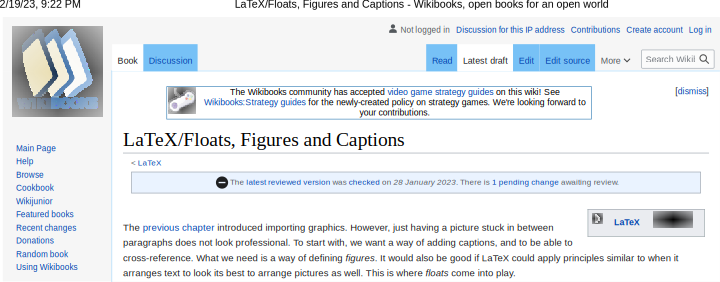
\includegraphics[width=0.8\textwidth]{wikibooks-figures.pdf}
    \caption[Wikibooks]{Screenshot der Wikibooks website \cite{figures}. Beachten
        Sie, dass der Text in dieser Grafik sogar selektierbar ist.}
    \label{fig:wikibooks}
\end{figure}

Dazu muss gar nicht viel gesagt, weil schon alles
auf Wikibooks \cite{figures} gefunden werden kann, 
wovon in \autoref{fig:wikibooks} ein
Screenshot zu sehen ist. Der \LaTeX-Code ist in 
\autoref{lst:figure-example} zu finden.

\subsection{\LaTeX-Code}
Zum Einbinden der \autoref{fig:wikibooks}
wurde der \LaTeX-Code im Listing 
\ref{lst:figure-example} verwendet.

\lstinputlisting[
label=lst:figure-example,
language=tex,
caption={Code zum Einbinden der \autoref{fig:wikibooks}.},
]{graphics-figure-example.tex}
 %        \
\chapter{Kompilierung}\label{sec:compilieren}

\section{Windows}\label{sec:windows}

Für Windows kann 
\href{https://tug.org/texlive/windows.html}{\TeX{}live} empfohlen werden,
Dowload auf \href{https://tug.org/texlive/windows.html}{\url{https://tug.org/texlive/windows.html}}

Normalerweise wird \LaTeX{} mit einem Texteditor geschrieben,
vorzugweise mit einem speziellen \LaTeX{}-Modus, oder gleich ein
spezialiserter Texteditor. \TeX{}live empfiehlt den \TeX{}works Editor,
zu finden auf 
\href{https://www.tug.org/texworks/}{\url{https://www.tug.org/texworks/}}.

Eine weitere Möglichkeit für eine LaTeX-Distribution
ist MiKTeX, die auch mit einem 
spezialisierten Editor geliefert wird. 

Es gibt auch ein <<Grafisches Interface>>,
\href{https://www.lyx.org/}{LyX (http://www.lyx.org)}. Was der taugt,
und ob das überhaupt empfehlenswert ist, kann ich nicht beurteilen.

\section{Mac}
Da gibt es offenbar \href{https://tug.org/mactex/}{MacTeX
  (https://tug.org/mactex/)}. Wird wohl gut sein.

\section{Cloud-Lösung Overleaf}
Cloud-Lösung für \LaTeX. Sorgen Sie für ein regelmässiges lokales
Backup (wie bei allen Cloud-Diensten sind Ihre Daten auf fremden Datenträgern).

\section{Linux}\label{sec:linux}
Für diese Vorlage wurde das Makefile in \autoref{lst:makefile} verwendet.

Sollte das Programm make nicht schon installiert sein, installieren Sie bitte das Ubuntu-Package 
<<build-essential>> (oder ähnliches).

\lstinputlisting[
	language=make,
	label=lst:makefile,
	caption={[Makefile]Das Makefile, das diese Dokument kompiliert.},
% linerange={88-93},firstnumber=88
]{Makefile}


Die einzelnen Kommandos können natürlich auch manuell eingegeben
werden. Gerade für grössere Projekte eignen sich Makefiles aber, da
alle Abhängigkeiten spezifiziert werden können. Z.B.\ können auch
programmatisch erzeugte Grafiken automatisch neu erstellt werden, wenn
die zugrundeliegenden Daten sich ändern.

 %     \
\chapter{Mathematik in \LaTeX}\label{sec:mathezeugs}

\section{Vektoren}

Es empfiehlt sich die <<amsmath>> package einzubinden, mit
\begin{verbatim}
\usepackage{amsmath}
\end{verbatim}

\begin{equation}\label{eq:erste}
\vec v = \begin{pmatrix}
a_1\\
a_2\\
a_3
\end{pmatrix}
\end{equation}

Verwendet man \autoref{eq:erste} dann erhält man:

\begin{equation}\label{eq:zweite}
\vec u = \begin{pmatrix}
a_1+b_1\\
a_2-\pi\\
a_3+\cos\left(\alpha^2\right)
\end{pmatrix}
\end{equation}

Den Code dazu ist in \autoref{fig:latex-code} ersichtlich.

\subsection{Code}
\begin{figure}[ht]
\centering
\begin{minipage}{0.8\textwidth}
\begin{verbatim}
\begin{equation}\label{eq:erste}
\vec v = \begin{pmatrix}
a_1\\
a_2\\
a_3
\end{pmatrix}
\end{equation}

Verwendet man \autoref{eq:erste} dann erhält man:

\begin{equation}\label{eq:zweite}
\vec u = \begin{pmatrix}
a_1+b_1\\
a_2-\pi\\
a_3+\cos\left(\alpha^2\right)
\end{pmatrix}
\end{equation}

Den Code dazu ist in \autoref{fig:latex-code} ersichtlich.

\end{verbatim}
\end{minipage}
\caption{Code zu \autoref{eq:erste} und \autoref{eq:zweite}}
\label{fig:latex-code}
\end{figure}
 %      \
\chapter{Massangaben}\label{sec:massangaben}

Sobald Masseinheiten angegeben werden, lohnt sich das package
{\tt siunitx}\cite{siunitx}.


\section{Beispiele}
Mehr Beispiele finden Sie in der offiziellen Dokumentation des package.
\begin{itemize}
	\item Beschleunigung $g = \qty{9.81}{\metre\per\square\second}$. 
	\verb+$g = \qty{9.81}{\metre\per\square\second}$+
%
	\item Strom $I = \qty{25}{\micro\ampere}$.
		\verb+$I = \qty{25}{\micro\ampere}$+
	\item Widerstand $R = \qty{2}{\mega \ohm}$.
		\verb+$R = \qty{2}{\mega \ohm}$+
\end{itemize}

\section{Alte Version (v2) von siunitx}
Sollte Ihr System noch eine alte Version von siunitx haben, verwenden Sie
anstatt \verb+\qty+ den Befehl \verb+\SI+, also z.B.

\verb+\SI{25}{\micro\ampere}  +
anstatt
\verb+   \qty{25}{\micro\ampere}+

Siehe auch \cite{qty-vs-si}.
 %      \
\chapter{Chemie}\label{sec:chemie}


\section{Packages}
Es gibt mehrere Packages. Exemplarisch ist hier das <<mhchem>>\cite{mhchem}
Package vorgestellt:

\begin{verbatim}
\usepackage[version=4]{mhchem}
\end{verbatim}

\section{Verwendung} \label{sec:chemie-verwendung}
Am besten lesen Sie die Dokumention des Packages, das ist voll mit vielen
Beispielen. Hier sind einige daraus:

\ce{H2O}

\ce{Na+} und \ce{Cl-}

\ce{^{227}_{90}Th}

Der entsprechende Code ist in \autoref{fig:chemie} zu finden.

\begin{figure}[ht]
\centering
\begin{minipage}{0.8\textwidth}
\begin{verbatim}
\ce{H2O}

\ce{Na+} und \ce{Cl-}

\ce{^{227}_{90}Th}
\end{verbatim}
\end{minipage}
\caption{\LaTeX{}-Code, der die chemischen Formeln in
	\autoref{sec:chemie-verwendung}
erzeugt.}
\label{fig:chemie}
\end{figure}
 %      \
\chapter{Einbinden von Code}\label{sec:code}
Vollständige Code-Listings gehören nicht in den Bericht, sondern auf
die dem Bericht beigelegte SD-Karte.

Schlüsselstellen in einem Programm machen aber durchaus Sinn,
aufgeführt zu werden.

Im \autoref{lst:javaquine} auf der nächste Seite ist das
Listing eines Quines abgebildet (ein Programm, das seinen eigenen Source-Code als
Ausgabe produziert).

\newpage

\lstinputlisting[
label=lst:javaquine,
caption={[JavaQuine]Ein Java Quine\cite{javaquine}},
% linerange={88-93},firstnumber=88
]{\codefile{Quine}}
 %            \
\documentclass{beamer}

\usepackage[german]{babel}        % Deutschsprachige Beschriftungen
\usepackage[utf8]{inputenc}       % Utf8 Zeichensatz
\usepackage{graphicx}             % Grafiken
\usepackage{fancyvrb}             % Für VerbatimInput




% See https://www.overleaf.com/learn/latex/Beamer#:~:text=package%20in%20Overleaf-,Reference%20guide,-Below%20is%20a
\usetheme{Warsaw}
\usecolortheme{default}

\beamertemplatenavigationsymbolsempty
\setbeamertemplate{footline}[frame number]

%Information to be included in the title page:
\title{\LaTeX{} für die Maturaarbeit}
\author{Ivo Blöchliger}
\institute{Kantonsschule am Burggraben}
\date{29. August 2023}
\logo{\includegraphics[width=1.5cm]{images/ksbg-logo-no-text.pdf}}

\begin{document}

\frame{\titlepage}

\begin{frame}
\frametitle{Übersicht}
\tableofcontents
\end{frame}

\begin{frame}
	\frametitle{Download der Software}
	\begin{block}{\LaTeX{} Distribution}
		Downalod von Mik\TeX
	\end{block}
	\begin{block}{Editor}
		Download von \TeX{}Studio
	\end{block}
	Links auf https://fginfo.ksbg.ch
\end{frame}

\section{Was ist \LaTeX{}?}
\subsection{Geschichte}
\begin{frame}
	\frametitle{\LaTeX{}?}
	\begin{block}{Aussprache}
		Leitägg (oder Leitäch)
	\end{block}
	\begin{block}{Ursprung}
		\TeX{}: Textsatzsystem für Mathematik, 
		1978, Donald Knuth \\ 
		$\quad$ Ziel: Typographisch einwandfreie Dokumente\\[2mm]
		\LaTeX{}: Sammlung von Macros
		1984, Leslie Lamport
	\end{block}
	\begin{alertblock}{\includegraphics[height=1em]{images/Laser-symbol.pdf}
		Warnung \includegraphics[height=1em]{images/Laser-symbol.pdf}}
		Worddokumente können nach längerer Verwendung von \LaTeX{} zu Augenkrebs
		führen.
	\end{alertblock}
\end{frame}



\subsection{Prinzip}
\begin{frame}
	\frametitle{Prinzip von \LaTeX}
	Beschreiben was, nicht wie.
	\begin{block}{Textdatei {\tt prinzip.tex}}
		\VerbatimInput{prinzip.tex}
	\end{block}
\end{frame}


\begin{frame}
	\frametitle{Automatisieren}
	\begin{itemize}
		\item Nummerierungen
		\item Verweise
		\item Verzeichnisse
		\item Formatierungen
	\end{itemize}
\end{frame}

\begin{frame}
	\frametitle{Nummerierungen}
	\begin{block}{$\backslash$label\{bla\} und $\backslash$autoref\{bla\}}
		$\backslash$label\{bla\} {\bf nach} nummererzeugendem Befehl:\\[3mm]
		\begin{quote}
			{\tt $\backslash$section\{Blah
			Blah\}$\backslash$label\{sec:bla\}}\\[3mm]

			{\tt In $\backslash$autoref\{sec:bla\} \ldots}
		\end{quote}
	\end{block}

	\begin{block}{Labelpräfixe}
		\begin{description}
			\item[Kapitel] {\tt ch:bla}\\
			\item[Abschnitte] {\tt sec:bla}\\
			\item[Abbildungen] {\tt fig:bla}\\
			\item[Gleichungen] {\tt eq:bla}\\
		\end{description}
	\end{block}
\end{frame}

\begin{frame}
	\frametitle{Mathematik}
	Mitternachtsformel, Gleichung \ref{eq:quadsol}:
\begin{equation}\label{eq:quadsol}
	x_{1,2} = \frac{-b \pm \sqrt{b^2-4ac}}{2a}
	\qquad b^2-4ac \geq 0,\, a \neq 0
\end{equation}

	\vspace{-6mm}
	\begin{block}{\LaTeX{} Code}
		\VerbatimInput{mathe.tex}
	\end{block}
\end{frame}

\subsection{Kompilierung}
\begin{frame}
	\frametitle{Kompilierung}
	\begin{block}{Erzeugen des Dokuments}
		\begin{enumerate}
			\item Textsatz, Nummerierung, Benötigte Verweise
			\item Evtl.\ Erzeugen des Literaturverzeichnisses
			\item Textsatz, Eintragen aller Verweise, Verzeichnisse
		\end{enumerate}
	\end{block}
	\begin{example}
		Nach dem ersten Durchgang:\\[2mm]
		\begin{quote}
			\rm
			{\large \bf Abschnitt 2.1}\\
			{Wie im Abschnitt ?? ersichtlich, \ldots}
		\end{quote}
	\end{example}
\end{frame}

\begin{frame}
	\frametitle{Automatisches Kompilieren}
	\begin{itemize}
		\item Mehrere Programme nötig
		\item Richtige Reihenfolge
	\end{itemize}
	\begin{block}{Automatisieren}
		\begin{itemize}
			\item TeXStudio (Editor)
			\item Visual Studio Code Plugin (?)
			\item Makefile (make)
		\end{itemize}
	\end{block}
\end{frame}

\subsection{Bilder}
\begin{frame}
	\frametitle{Bilder}

	\begin{block}{Vektoriell bitte!}
		Wenn irgendmöglich vektorielle Bilder verwenden:
		\begin{itemize}
			\item SVG $\leftarrow$ PDF
			\item PDF (wenn nicht einfach Pixelbild)
		\end{itemize}
		Aus Office-Anwendungen: {\bf Print as PDF...}
	\end{block}
	\begin{block}{Wenn Pixel, dann}
		\begin{description}
			\item[PNG] Screenshots, Bilder mit einfarbigen Flächen
			\item[JPG] Photos
		\end{description}
	\end{block}
\end{frame}

\begin{frame}
	\frametitle{Vergleich der Formate}
	\begin{columns}[onlytextwidth]
		\begin{column}{0.33\textwidth}
		  \centering
			PDF (5.5 kB)\\[5mm]
			
\includegraphics[width=\textwidth]{images/vektor.pdf}
		\end{column}
		\begin{column}{0.33\textwidth}
		  \centering
			 PNG (21 kB)\\[5mm]
			
\includegraphics[width=\textwidth]{images/vektor.png}
		\end{column}
		\begin{column}{0.33\textwidth}
		  \centering
			JPG (17 kB)\\[5mm]
			
\includegraphics[width=\textwidth]{images/vektor.jpg}
		\end{column}
	\end{columns}
\end{frame}

\begin{frame}
	\frametitle{Platzierung automatisch, nicht im Textfluss}
	\begin{block}{Gründe}
		\begin{itemize}
			\item Konzipiert für wissenschaftliche Publikation
			\item Abbildungen speziell farbig, eigene Seiten
			\item Layout dem Autor nicht bekannt
			\item Rücksicht auf Textfluss, Seitenfüllung
		\end{itemize}
	\end{block}
	\begin{alertblock}{Nummerieren, referenzieren!}
		\begin{itemize}
			\item Alle Abbildungen sind nummeriert,\\
		 	\item mit Legende versehen\\
			\item und {\bf im Text referenziert}.
		\end{itemize}
	\end{alertblock}
\end{frame}


\section{Software}
\subsection{Absolut nötige Software}
\begin{frame}
	\frametitle{Benötigte Software}
	\begin{itemize}
		\item \LaTeX{} Distribution (z.B. MikTeX oder TeXLive)
			\begin{itemize}
				\item Programme: {\tt pdflatex}, {\tt bibtex}, {\tt biber}, etc.
				\item \LaTeX{} Pakete: {\tt beamer}, {\tt babel}, {\tt graphicx}, etc.
			\end{itemize}
		\item Texteditor: TeXStudio, Visual Studio Code, Vim, \ldots
		\item PDF-Viewer
	\end{itemize}
\end{frame}

\subsection{Nützliche Software}
\begin{frame}
	\frametitle{Nützliche Software}
	\begin{itemize}
		\item Inkscape, LibreOffice (SVG, PDF)
		\item make o.ä. als Buildsystem
		\item Verzeichnisse/Konverter zu Bib\TeX{} Einträgen
		\item Erstellung von \LaTeX{}-Tabellen
	\end{itemize}
\end{frame}



\section{Hilfe!}
\begin{frame}
	\frametitle{Hilfe!}
	\begin{block}{Tech-Lab (E23)}
		Dienstags ab 16:40\\
		Freitags ab 17:20
	\end{block}
	\begin{block}{Teams}
		Fragen und Antworten auf dem \LaTeX{} Team
	\end{block}
	\begin{block}{Vorlage auf Github}
		Ergänzungen, Verbesserungen gerne liefern!
	\end{block}
\end{frame}

\begin{frame}
	\frametitle{Dank}
	\centering
	\Huge
	Herzlichen Dank\\
	für Ihre Aufmerksamkeit\\[1cm]
	Fragen?
\end{frame}

\begin{frame}
	\frametitle{Weiteres Vorgehen}
	\begin{block}{Plan}
		\begin{itemize}
			\item Software installieren
			\item Vorlage herunterladen
			\item Vorlage kompilieren
			\item Minimalbeispiel kompilieren
			\item Minimalbeispiel studieren/ändern
		\end{itemize}
	\end{block}
\end{frame}

\end{document}

\chapter*{Dank}
Ich darf hier wieder <<ich>> schreiben, und ich möchte Luca Bosin ganz herzlich
dafür danken, dass ich diese Vorlage auf Basis seiner Maturaarbeit anpassen
durfte und dabei gleich noch einige Neuerungen entdecken durfte, insbesondere
die verbesserte Literaturverzeichniserstellung mit biber.



% --------------------------

% === Optional: INDEX ====
\cleardoublepage  %      \  
\phantomsection %        \
\addcontentsline{toc}{chapter}{\indexname} 
\printindex %            \
% ------------------------


% === ABBILDUNGSVERZEICHNIS ===
\cleardoublepage %             \
\phantomsection %              \
\addcontentsline{toc}{chapter}{\listfigurename}
\listoffigures %               \
% -----------------------------

% === CODEBLOCKVERZEICHNIS ===
\cleardoublepage %            \
\phantomsection %             \
\addcontentsline{toc}{chapter}{\lstlistlistingname}
\lstlistoflistings %          \
% ----------------------------

% === LITERATURVERZEICHNIS ===
\cleardoublepage %            \
\phantomsection %             \
\addcontentsline{toc}{chapter}{\bibname}
\printbibliography %          \
% ----------------------------



% =========== START VON ANHÄNGE ===========
\appendix

% === EIGENSTÄNDIGKEITSERKLÄRUNG ===
\chapter{Eigenständigkeitserklärung}\label{ch:appendix_independencedeclaration}
{\Huge ACHTUNG: Version vom 2018. Bitte den aktuellen Vorgaben
entsprechend anpassen!}

<<Ich bestätige mit meiner Unterschrift, dass ich meine Maturaarbeit selbständig verfasst und in schriftliche Form gebracht habe, dass sich die Mitwirkung anderer Personen auf Beratung und Korrekturlesen beschränkt hat und dass alle verwendeten Unterlagen und Gewährspersonen aufgeführt sind. Mir ist bekannt, dass eine Maturaarbeit, die nachweislich ein Plagiat gemäss der in der Maturaarbeitsbroschüre gegebenen Definition darstellt, als schwerer Verstoss im Sinne des Maturitätsprüfungsreglements gewertet wird.>>

\vspace{3cm}

\noindent
\begin{tabular}{p{0.47\linewidth}p{0.47\linewidth}}
  Ort \&\ Datum & Unterschrift \\
  & \\[1cm]
  \hline
\end{tabular}

% ----------------------------------

% =========== ENDE VON ANHÄNGE ============



% =============================================================
\end{document} % ENDE VOM DOKUMENT ============================
% =============================================================
